% Page 040 — page imprimée 36
% Contenu seul : le préambule, l'en-tête et la pagination sont gérés par meyrueis.tex

Cinquante six ans plus tard en 1977, lors d’une courte visite à Meyrueis, j’essayai de retrouver
la bergerie. Le chemin existait toujours quoique embroussaillé mais le petit champ était
clôturé et avait une porte neuve fermée à clé. Et la tranchée qui menait à l’entrée de la grotte
avait été soigneusement remplie sur toute sa longueur par des branchages aux épines acérées.

Ma grotte était condamnée, plus dangereuse peut-être que je ne l’avais cru. Dommage ...

J’aurais aimé pouvoir retrouver, ne fut-ce que pour un moment, l’obscurité totale et le
silence, un silence ponctué depuis toujours par la chute d’une goutte d’eau dans une vasque..
la même... jamais la même ! ».

\begin{center}
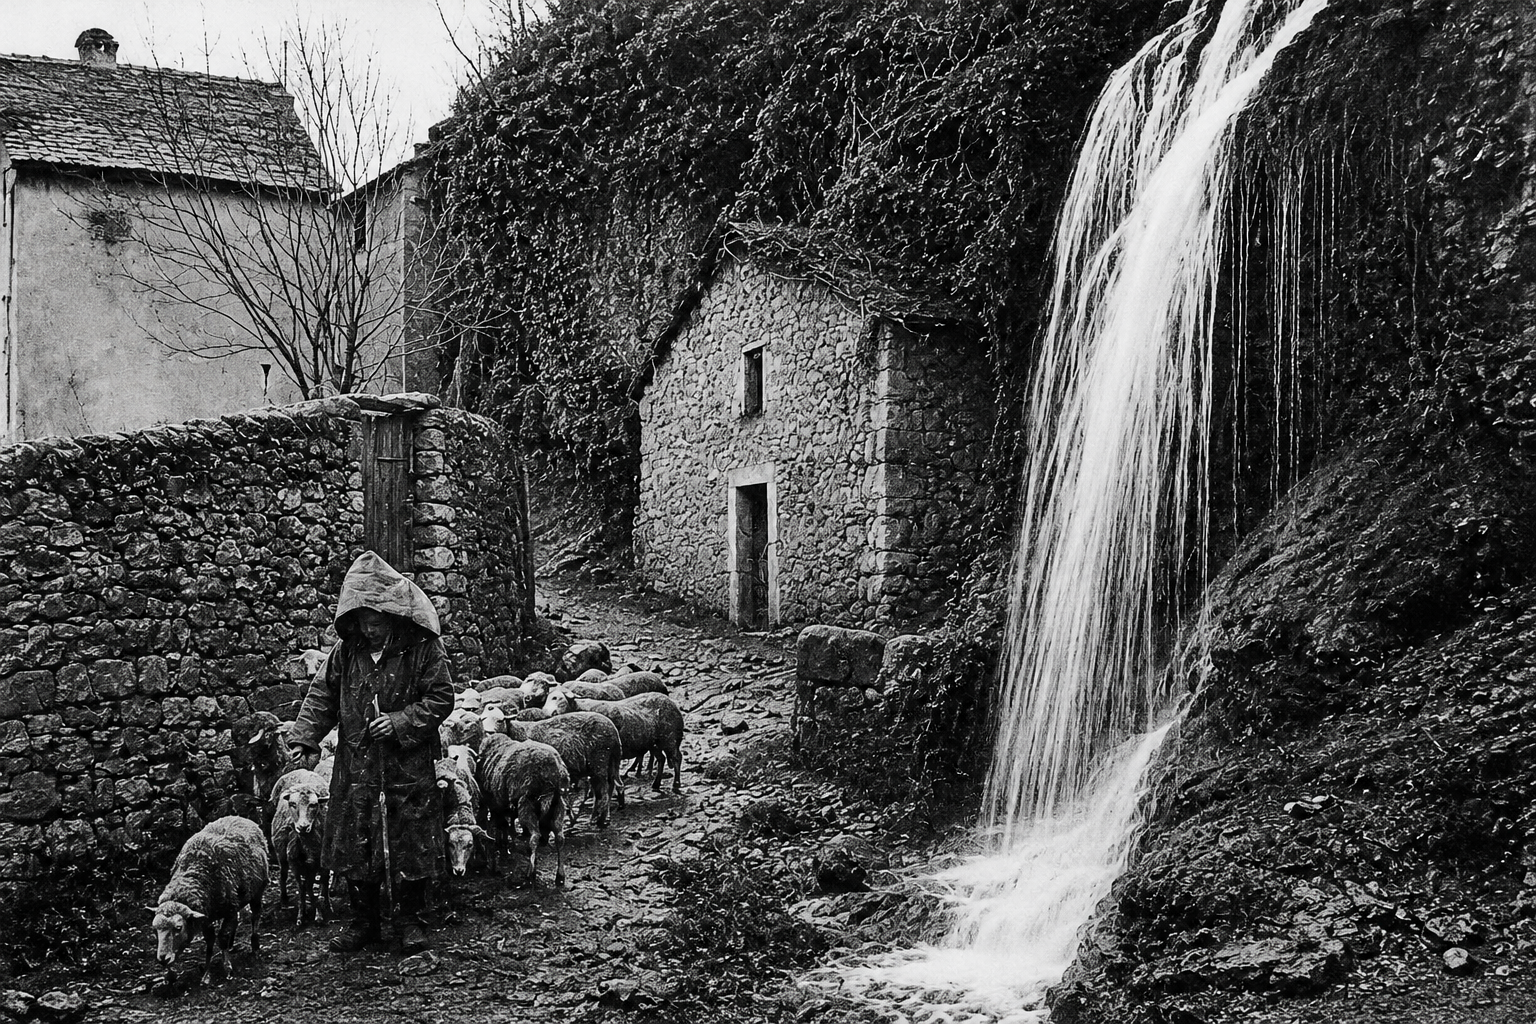
\includegraphics[width=0.78\textwidth]{imgs/040.png}
\end{center}
